% !TEX TS-program = XeLaTeX
% !TEX encoding = UTF-8 Unicode

\chapter{工程应用}

\label{chap04}

\section{工程背景} 
内蒙古自治区鄂尔多斯市是我国重要的能源基地,
已探明的天然气储量约1880亿立方米,约占全国总储量的三分之一,
已探明的煤炭储量1496亿多吨,约占全国总储量的六分之一。
鄂尔多斯的煤炭资源不仅储量大、分布广,而且品种齐全,
有褐煤、长焰煤、不粘结煤、弱粘结煤、气煤、肥煤、焦煤等,
并且大多埋藏浅,垂直厚度深,易开采。

位于鄂尔多斯市的某煤矿是一座新建的年产千万吨的现代化煤矿。
从2010年开始试运营。试运营开始时已建设完成完善的生产生活设施,
专用铁路也正在建设。
该煤矿同时建设有一个洗煤厂,可以满足整个煤矿最大生产能力时的需求。
同时为了在生产、加工、运输、销售等环节间进行有效的缓存,共建设了10个煤仓。
其中有原煤仓两个,矸石仓两个、块煤仓4个、末煤仓2个。
下图(\ref{figure:xiaoguotu})即为该煤矿的效果图。
\begin{figure}[!htbp]
   \centering
   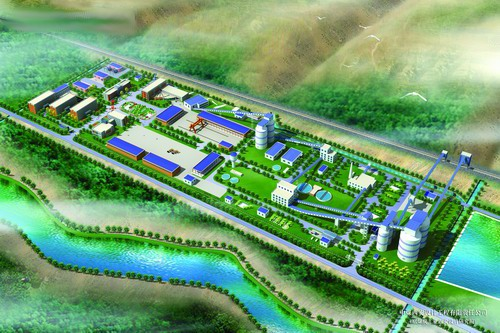
\includegraphics[scale=0.7]{xiaoguotu.jpg}
   \bicaption[figure:xiaoguotu]{厂区效果图}{厂区效果图}
								{Fig.}{Factory renderings}
\end{figure}

矿井生产出的煤炭通过皮带直接运入原煤仓。
经过原煤仓缓存之后,进入洗煤厂进行加工。
经洗煤厂筛选,分选出矸石、块精煤、末煤等,分别进入各自的煤仓。
最后通过各煤仓附属的装载设备,装载到汽车、火车运往各地。

在这些煤仓中,储煤量最大的是两个末煤仓,均可装载2.5万吨煤。
其次是原煤仓,每个装载能力为1万吨。
另外,块精煤仓和矸石仓的装载能力分别为2500吨和1000吨。

根据该煤矿的实际情况,末煤仓的装载能力最大,
日常运营中和使用中装载的煤炭量也最大,因此对地面的压力也最大,
是最需要特别关注的。上图(\ref{figure:xiaoguotu})中,
最大的两个煤仓即为末煤仓。

\section{观测方法}
鉴于煤仓对于安全、有效生产的重要性,在施工过程中和投产使用后,
必须进行沉降观测,以便掌握其沉降情况,及时发现对煤仓运营不利的下沉,
提前采取措施,保证煤仓的安全使用,同时也为今后合理设计提供资料。
本文所提沉降观测仅涉及投产使用后的沉降观测。

本工程的沉降观测采用精密水准测量方法,使用的仪器为徕卡DNA03电子水准仪。

\subsection{水准控制网的布设}
建筑物沉降观测的依据是埋设在建筑物附近的水准点,即基准点。
为了在各基准点之间相互校核并防止因为某个基准点的高程变动而造成基准的错误,
至少埋设三个基准点。
这些控制点应该埋设在建筑物、构筑物基础压力影响范围以外,
避免对沉降原因的判断产生错误;
同时也应该在锻锤、轧钢机、铁路、公路等震动影响范围以外;
并且也要远离地下管道;埋设深度至少要低于冰冻线及地下水位变化范围0.5m。
水准点离开观测点不应太远,以免因为线路过长影响精度。

沉降观测开始时,厂区仍然在进行着频繁的施工建设。
鉴于这种情况,控制网可以按照两级布设。
在厂区外的合适地点,布设第一级控制网,以保证这些点能够稳定,
不受厂区内施工的影响,也不受到采煤的影响。
同时为了观测的方便,在厂区内,布设第二级控制网,
这些控制点的位置应该选择在离各个煤仓位置相对较近、
受施工影响可能比较小、地面条件较稳定的地点。

第一级控制网和第二级控制网要定期进行联测,以检测第二级控制网的稳定性。
联测应该严格按照国家二等水准测量的规范要求进行。
如果第二级控制网发生了变化,要及时采取对控制点进行加固、布设新的控制点、
对控制点高程加常数等措施进行处理,并考虑修正前期煤仓沉降观测值。

(***)国家及行业有关规范标准均规定,
沉降观测点的布设应结合地质情况及建筑物结构特点,
以能全面反映建筑物地基变形特征来确定。
从平面设置考虑, 沉降观测点一般布设在建筑物的四角、转角、
沿外墙 每$10\sim15m$处或每隔$2\sim3$根立柱的柱基上。
从纵向设置考虑,沉降点一般布设在主体的
$± 0.00$以上$0.5m$左右的外墙上较合适,这样观测时立尺、观测均较方便。
建设煤仓时,已经在比较容易到达的地方,预设了四个对称的沉降观测目标点。
通过这四个对称的目标点,既可以检测出煤仓整体的沉降情况,
也可以监测到煤仓可能发生的倾斜情况。

以上所有的第一、第二级控制点,煤仓上的沉降目标点,都需要随时注意保护,
如果发现发生变化或者损坏,需要随时修复并重测,
或者重新布设受损的控制点和目标点。

\subsection{观测时间}
对于煤仓的观测一般采用定期观测的方法。
煤仓刚刚投入使用时,观测的密度需要更加频繁,
随着使用时间的推移,观测密度也随之减小。
在根据周期进行观测的同时,同时也需要注意煤仓的装载量。
如果装载量在短时间内有较大的变化,也需要增加观测,以保证安全。

\subsection{精度选择}
为了能够确保检测出煤仓沉降的变化,需要对观测的精度提出限定。
对观测基准点进行联测时,需要满足国家二等精密水准观测的规范要求,
以保证观测的准确性和可靠性。

在使用基准点对煤仓上的沉降点进行观测时,
对于闭合差、前后视距差等参数的要求严格参考国家二等水准测量的规范要求,
但是并不进行往返测量,
对于其它一些确有困难且并不是特别重要的参数也可以适当放宽要求。
\begin{figure}[!htbp]
   \centering
   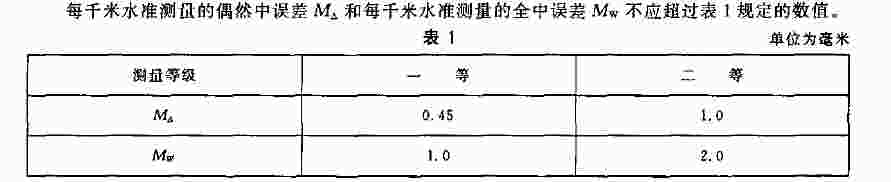
\includegraphics[scale=0.5]{level2requirement1.jpeg}
   \bicaption[figure:error-per-km]{每千米中误差要求}{每千米中误差要求}
								{Fig.}{Error per KM}
\end{figure}

\begin{figure}[!htbp]
   \centering
   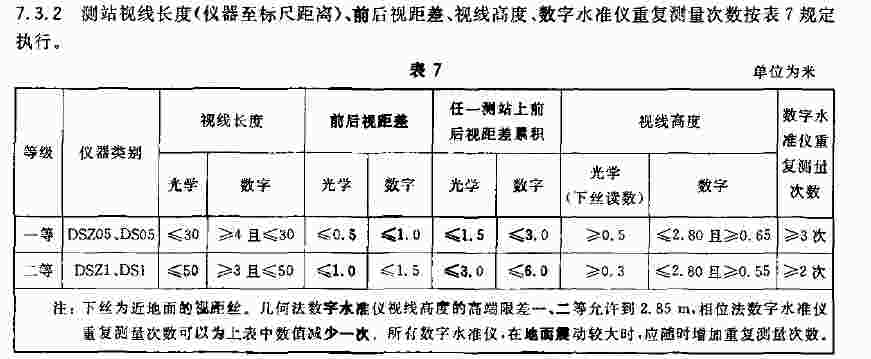
\includegraphics[scale=0.5]{level2requirement2.jpeg}
   \bicaption[figure:line-of-sight]{视线和重复测量要求}{视线和重复测量要求}
						{Fig.}{Line of sight and repeated measurements}
\end{figure}

\begin{figure}[!htbp]
   \centering
   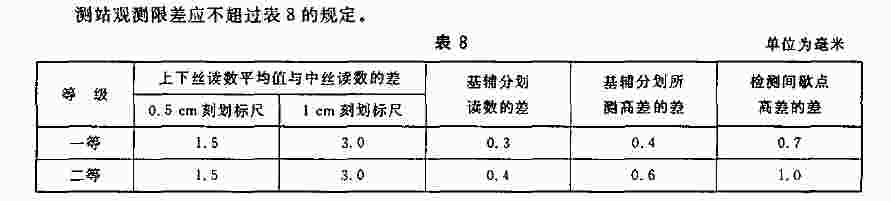
\includegraphics[scale=0.5]{level2requirement3.jpeg}
   \bicaption[figure:b-a-part]{基辅分划读数限差}{基辅分划读数限差}
								{Fig.}{Basic and auxiliary partition}
\end{figure}

\begin{figure}[!htbp]
   \centering
   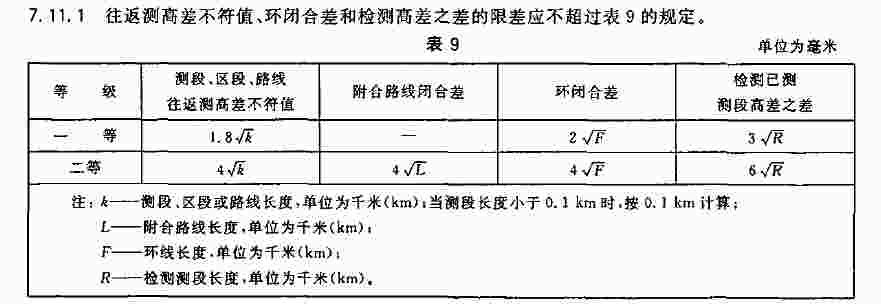
\includegraphics[scale=0.5]{level2requirement4.jpeg}
   \bicaption[figure:go-return]{往返高差不符值、环闭合差、检测高差之差的要求}{往返高差不符值、环闭合差、检测高差之差的要求}
			{Fig.}{Difference of going and forth, Misclosure, Check}
\end{figure}

\newpage
\subsection{预警处理}
当煤仓观测过程中沉降值或者沉降速率超出预警值或者发现煤仓出现倾斜时,
必须立即报告煤仓的使用单位,同时应及时增加观测或着调整观测方案。
同时如果在观测过程中出现煤仓周围进行开挖等作业时,也需要增加观测次数。
另外,如果煤仓周围出现暴雨、爆炸或者地震等特殊情况时,也应该增加观测次数。


\section{数据处理}
外业观测试验徕卡DNA03电子水准仪进行,观测的数据也同时存储在电子水准仪中。
内业时,使用LEICA Geo Office软件处理提取出各个观测点的高程值。
将这些观测到的高程值,写入逗号分隔的文本文件(.CSV),
文件中的字段均不加引号,编码使用UTF-8编码。
最后通过使用Python编写的程序,生成HTML格式的各种统计表格以及沉降曲线。

\subsection{原始数据文本数据库}
外业收集的原始数据分为装载量、观测高程、注释和点所属煤仓名等,
将它们分别放置在多个文件中。
建立四个数据文件,分别对应着原煤仓,矸石仓,块精煤仓和末煤仓的沉降数据。
各个文件中,煤仓沉降点名按照煤仓类型统一编号。

1)装载量数据文件的格式为:第一行为观测日期,第二行为观测者姓名,
第三行为数据计算者姓名,
第四行及以下为各个煤仓的装载量(装载量占总装载能力的百分比)。
每个字段均不加引号。
\begin{figure}[!htbp]
   \centering
   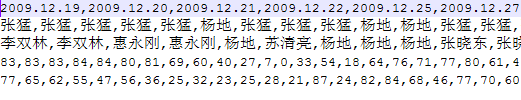
\includegraphics[scale=0.5]{4-heavy-csv.png}
   \bicaption[figure:4-heavy]{装载量文本数据库格式}{装载量文本数据格式}
			{Fig.}{Format of text-database for load}
\end{figure}

高程观测值文件的格式同样也是逗号分隔的文本文件,其格式为:第一行是观测日期,从第二行起是煤仓上各沉降点的高程观测值。
\begin{figure}[!htbp]
   \centering
   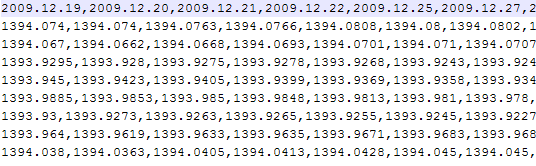
\includegraphics[scale=0.5]{4-level-csv.png}
   \bicaption[figure:4-level]{高程值数据文件格式}{高程值数据文件格式}
			{Fig.}{Format of text-database for leveling}
\end{figure}

注释文件的格式与高程观测值文件的格式完全相同,
但是如果遇到某个数据与高程观测值文件中对应的文件不同,
注释文件中的此数据在生成报表文件时将会作为注释对待。

\newpage
点号文件存储了每个煤仓上沉降点的信息。
第一列是煤仓类型的编号,依次为一号原煤仓、二号原煤仓、一号矸石仓等。
第二列及后面各列是每个煤仓上沉降点的编号。
\begin{figure}[!htbp]
   \centering
   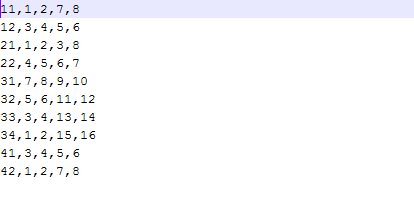
\includegraphics[scale=0.5]{static-csv.png}
   \bicaption[figure:static-csv]{点号数据库格式}{点号数据库格式}
			{Fig.}{Format of text-database for point number}
\end{figure}

\subsection{生成的报表以及图像}
根据观测数据文件,使用Python编程语言编写报表生成程序,
生成了几种需要的报表格式以及沉降曲线。

单点沉降值表,包括序号、时间、本次下沉、累积下沉、高程、
载荷、观测者、计算者、备注共10项。这个表格的每一行表示一次观测。
\begin{figure}[!htbp]
   \centering
   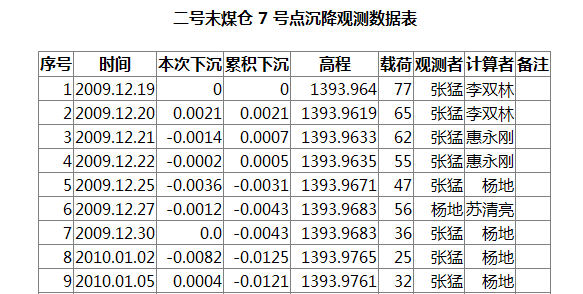
\includegraphics[scale=0.5]{42-7-all.png}
   \bicaption[figure:set-for-single]{单点沉降报表}{单点沉降报表}
			{Fig.}{Report for single point}
\end{figure}

\newpage
煤仓各点高程表,总结煤仓上各点的高程观测值。
\begin{figure}[!htbp]
   \centering
   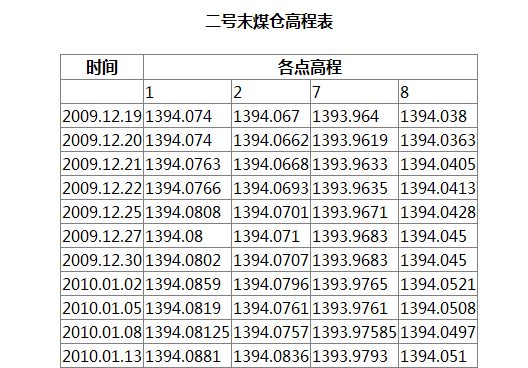
\includegraphics[scale=0.5]{42-new-level.png}
   \bicaption[figure:level-for-bunker]{煤仓上各点高程观测值}
					{煤仓上个点高程观测值}
			{Fig.}{Leveling of points in 1 bunker}
\end{figure}

煤仓各点沉降表,总结煤仓上各点的沉降值。
\begin{figure}[!htbp]
   \centering
   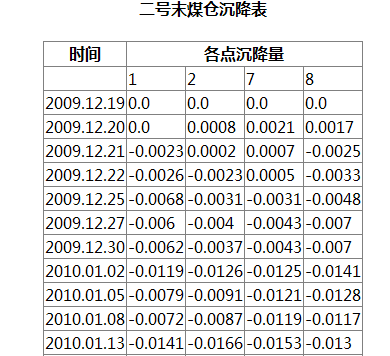
\includegraphics[scale=0.5]{42-settle.png}
   \bicaption[figure:level-for-bunker]{煤仓上各点沉降量}
					{煤仓上各点沉降量}
			{Fig.}{Settlement of points in 1 bunker}
\end{figure}
\newpage

沉降观测阶段总结表模板,根据命令行参数,生成需要提交的阶段总结模板,
经过适当的修改后,提交给委托方。
\begin{figure}[!htbp]
   \centering
   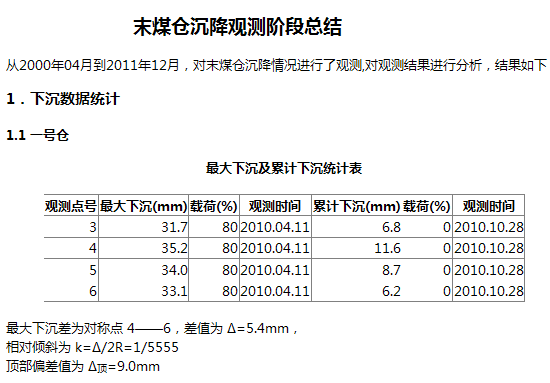
\includegraphics[scale=0.5]{4-paper.png}
   \bicaption[figure:paper]{阶段总结模板}
				    {阶段总结模板}
			{Fig.}{Template for periodic reports}
\end{figure}

沉降曲线图,横轴为从开始测量至最后一次测量的天数;
纵轴正方向为装载量,负方向为各点沉降量。
\begin{figure}[!htbp]
   \centering
   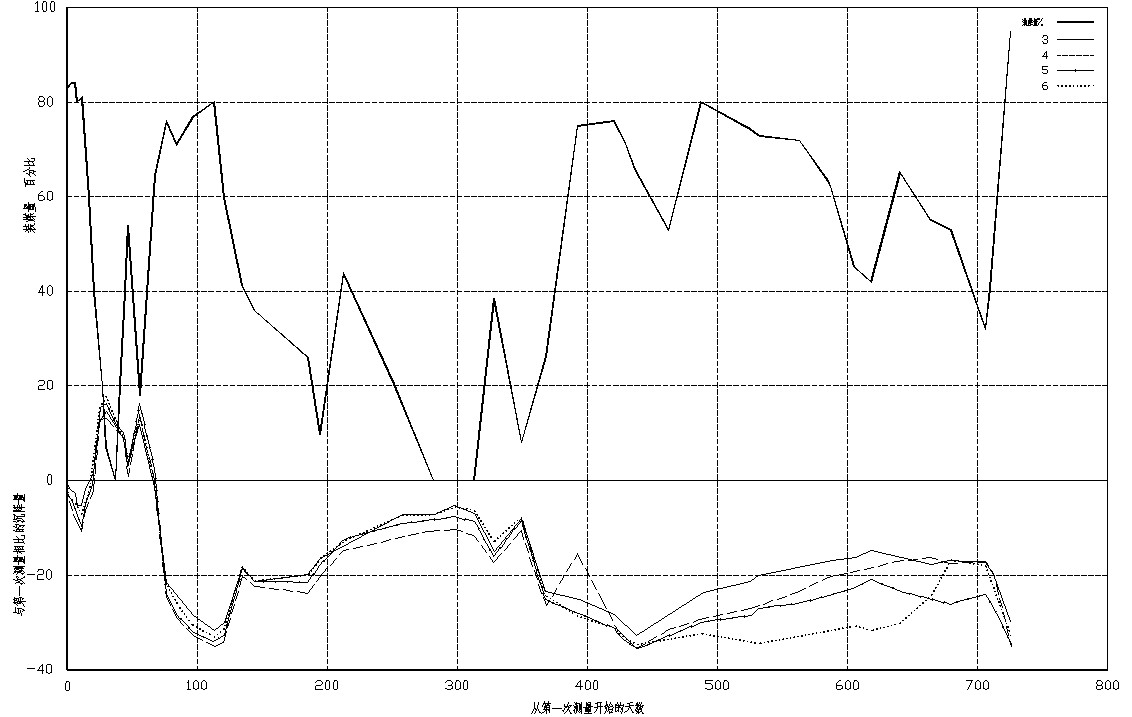
\includegraphics[scale=0.3]{41-plot.png}
   \bicaption[figure:plot-41]{一号末煤仓沉降曲线图}
				    {一号末煤仓沉降曲线图}
			{Fig.}{Curves for settlement fof Powder Bulker No.1}
\end{figure}

\begin{figure}[!htbp]
   \centering
   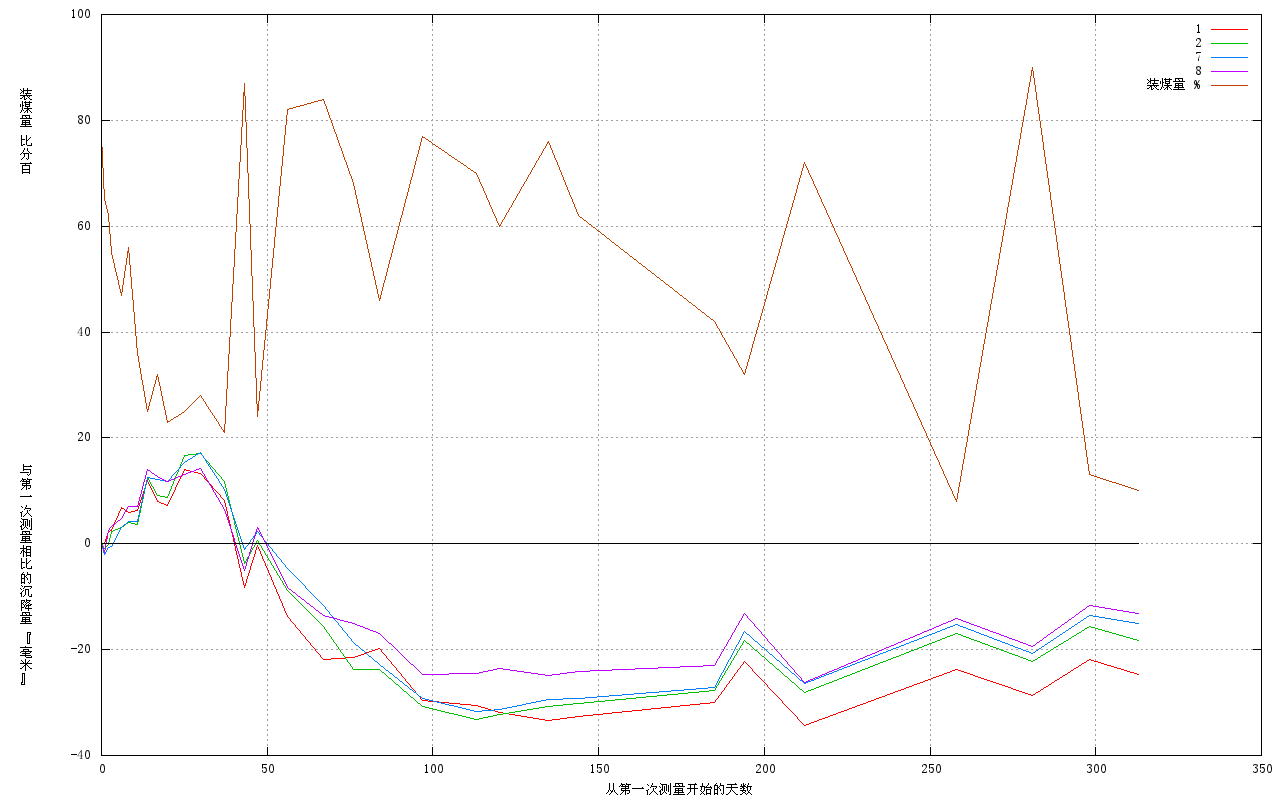
\includegraphics[scale=0.3]{42-plot.png}
   \bicaption[figure:plot-42]{二号末煤仓沉降曲线图}
				    {二号末煤仓沉降曲线图}
			{Fig.}{Curves for settlement of Powder Bulker No.2}
\end{figure}

\section{FastICA}
FastICA是一种流行的高效的独立成分分析算法,
是赫尔辛基理工大学的Aapo Hyvärinen发明。
该算法基于定点迭代方法,并以最大非高斯性作为统计独立性标准。
FastICA也可以导出相应的牛顿迭代方法。

其中一个单元的FastICA算法为(Wikipedia ***):\\
	1. 选择初始向量$W$ \\
	2. 令 $\bm{w}^{+} \quad \leftarrow 
			\quad E\{\bm{x}g(\bm{w^Tx})\} - E\{g'(w^Tx)\}w$ \\
	3. 令 $\bm{w} \quad \leftarrow \quad 
			\bm{w}^{+}/||\bm{w}^{+}||$ \\
	4. 如果未达到收敛要求,继续第2步 \\
此迭代算法求使数据$X$的投影达到最大高斯性的权向量W的方向。
函数$g()$是一个非二次的非线性函数的导数。
例如$g(t)$可是是$f(t)=t^4$的导数。

赫尔辛基理工大学信息和计算机科学实验室的研究人员
基于Matlab和GNU Octave开发了官方FastICA实现,
拥有易用的图形界面和计算功能强大的算法。
除此之外还有R语言、C++、Python等语言的实现。

MDP(Modular toolkit for Data Processing)是
一个基于Python的数据处理框架,
提供了丰富强大的数据处理功能,其中就包括FastICA和PCA。
本文即使用了MDP。

使用FastICA对一组数据进行分析的方法一般有两种:
直接使用FastICA算法,得到和原始数据同样数量的独立成分;
也可以首先使用主成分分析(PCA)对数据进行降维处理,
再使用FastICA进行分析。   

为了评估应用独立成分分析的效果,
可以使用Pearson相关系数、互信息和灰关联度作为评价指标。
计算得到的各独立成分与疑为影响因子之间的
Pearson相关系数、互信息和灰关联度,
根据这些关联性指标分析分离效果以及各种因素对煤仓沉降的影响。

\subsection{直接使用FastICA}
以末煤仓为例,将煤仓上4个点的观测序列分别作为原始信号,
直接使用MDP中的fastica函数进行分析,得出4个独立成分。

MDP中fastica函数原型是:
\begin{lstlisting}[language=Python, basicstyle=\ttfamily]
fastica(x, **kwargs)
\end{lstlisting}
其中的$x$为输入的原始信号,$kwargs$是在分离时使用的参数。\\
可以使用的参数及其默认值为
\begin{lstlisting}[language=Python, basicstyle=\ttfamily]
approach='defl', g='pow3', guess=None, fine_g='pow3', mu=1, 
stabilization=False, sample_size=1, fine_tanh=1, fine_gaus=1,
max_it=1000, max_it_fine=100, failures=5, limit=0.001, 
verbose=False, whitened=False, white_comp=None, white_parm=None,
input_dim=None, dtype=None
\end{lstlisting}
具体每个参数的定义请参考MDP的相应文档(***)。

该处直接使用默认参数,即:
\begin{lstlisting}[language=Python, basicstyle=\ttfamily]
fastica(x)
\end{lstlisting}
如下图像为,使用FastICA之后,根据得到的数据得到的,
观测值的图形见图(\ref{figure:plot-41})和(\ref{figure:plot-42})。

%一号末煤仓使用FastICA后得到的四个独立分量及装载量、气温的图像:
\begin{figure}[!htbp]
   \centering
   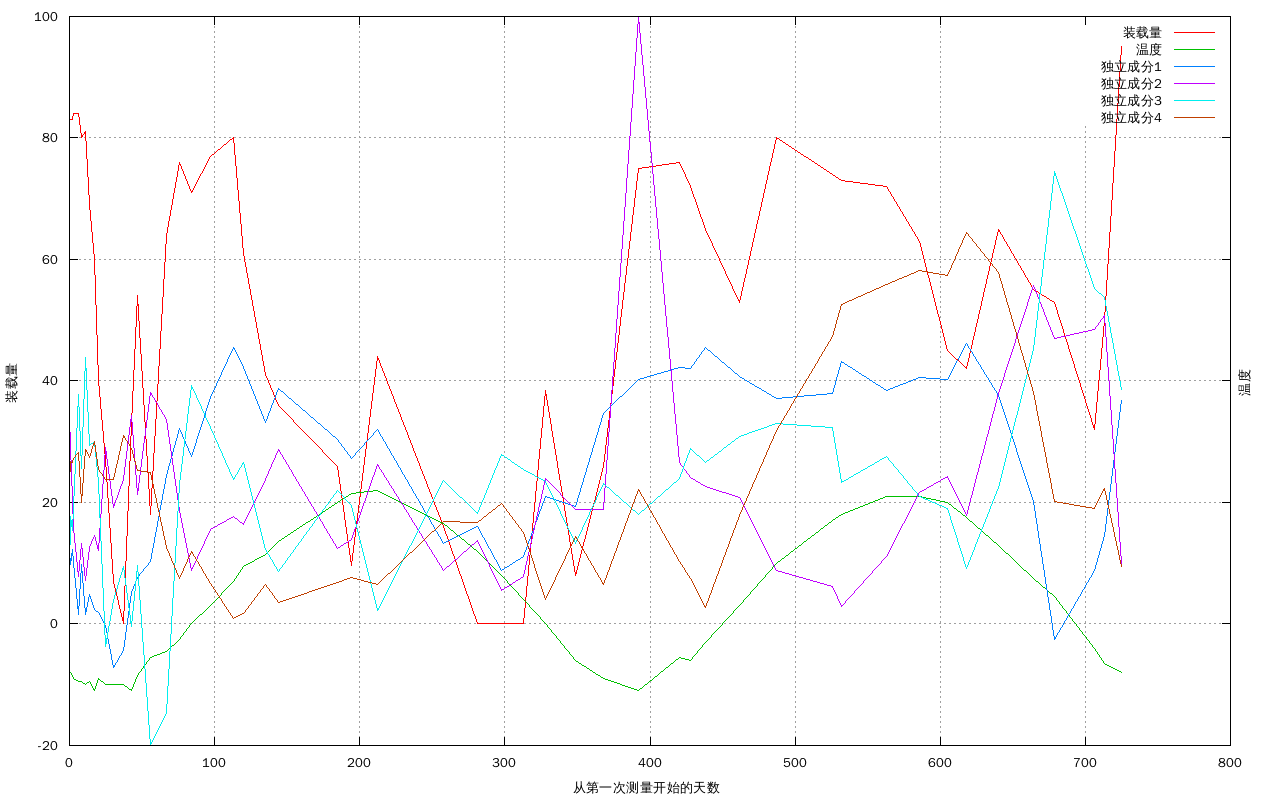
\includegraphics[scale=0.3]{41-ica-plot.png}
   \bicaption[figure:plot-41-ica]{一号末煤仓使用FastICA后得到的四个独立分量及装载量、气温的图像}
				    {一号末煤仓使用FastICA后得到的四个独立分量及装载量、气温的图像}
			{Fig.}{Four IC, Loadage and Temperature for Powder Bulker No.1}
\end{figure}

%二号末煤仓使用FastICA后得到的四个独立分量及装载量、气温的图像:
\begin{figure}[!htbp]
   \centering
   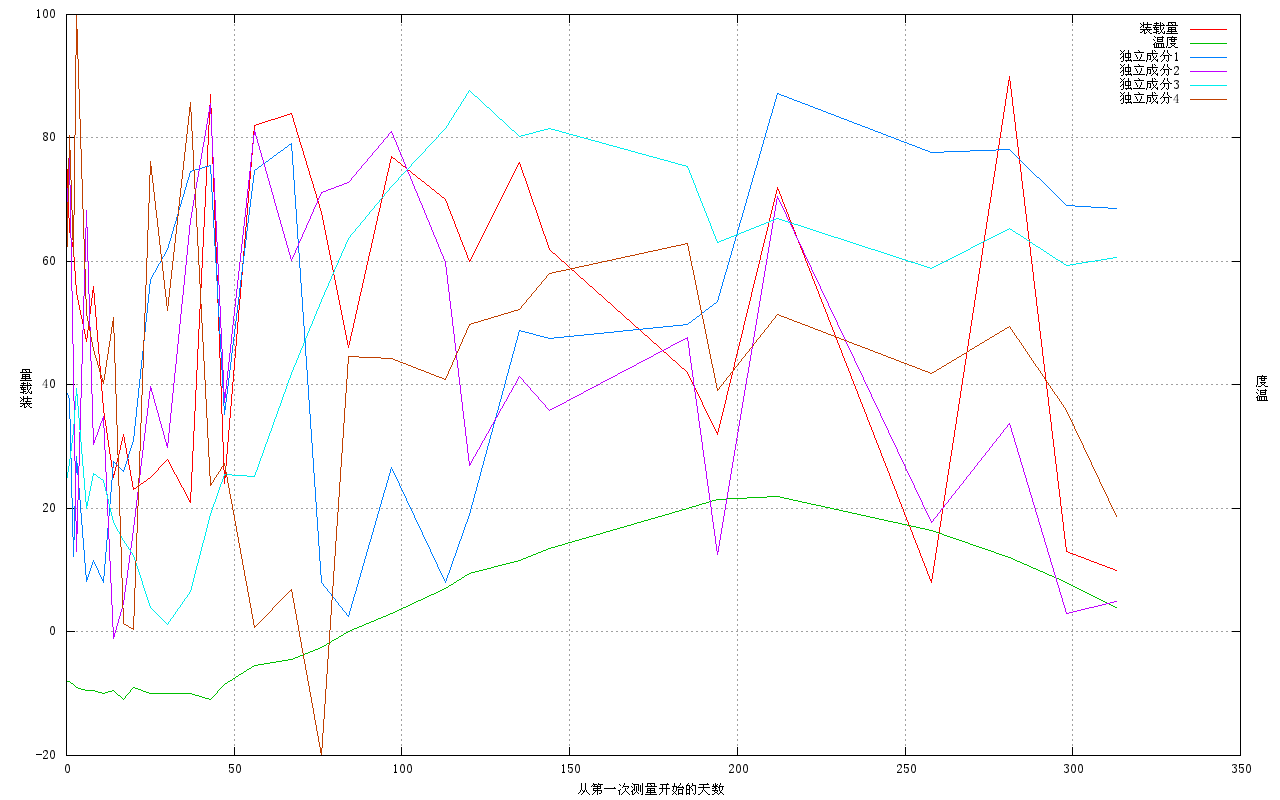
\includegraphics[scale=0.3]{42-ica-plot.png}
   \bicaption[figure:plot-42-ica]{二号末煤仓使用FastICA后得到的四个独立分量及装载量、气温的图像}
				    {二号末煤仓使用FastICA后得到的四个独立分量及装载量、气温的图像}
			{Fig.}{Four IC, Loadage and Temperature for Powder Bulker No.2}
\end{figure}


\subsection{首先使用PCA降维再应用FastICA}
MDP中也带了pca函数,可以用来对信号进行降维。
pca函数的原型是:
\begin{lstlisting}[language=Python, basicstyle=\ttfamily]
pca(x, **kwargs)
\end{lstlisting}
其中,$x$是需要进行主成分分析的信号,
$kwargs$是传递给pca函数的参数,
其可用的参数及其默认值有:
\begin{lstlisting}[language=Python, basicstyle=\ttfamily]
input_dim=None, output_dim=None, dtype=None, svd=False, 
reduce=False, var_rel=1e-12, var_abs=1e-15, var_part=None
\end{lstlisting}
关于具体的使用说明,请参考MDP的文档。
这里我们需要指定输入和输出的信号的维数:
\begin{lstlisting}[language=Python, basicstyle=\ttfamily]
pca(x, input_dim=4, output_dim=3)
\end{lstlisting}
此处我们设定输入的信号维数为4,输出的为3,
以和可能的影响因素的个数相同。
使用PCA对原始信号降维之后,再使用fastica函数获取独立分量。

以下对PCA降维后获得的数据使用fastica之后,画出的图像。
观测值的图形见图(\ref{figure:plot-41})和(\ref{figure:plot-42})

%一号末煤仓使用PCA+FastICA后得到的四个独立分量及装载量、气温的图像:
\begin{figure}[!htbp]
   \centering
   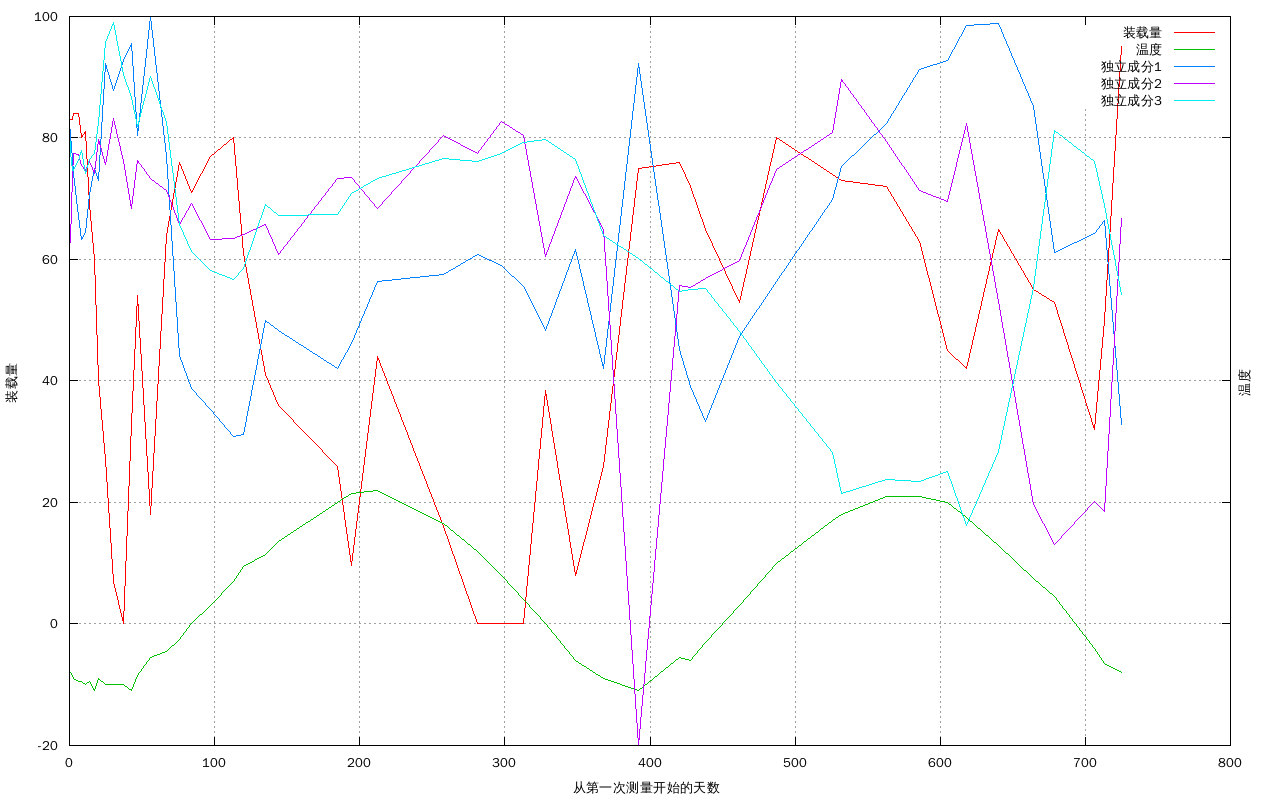
\includegraphics[scale=0.3]{41-pca-plot.png}
   \bicaption[figure:plot-41-pca]{一号末煤仓PCA降维后使用FastICA后得到的四个独立分量及装载量、气温的图像}
				    {一号末煤仓使用PCA降维FastICA后得到的四个独立分量及装载量、气温的图像}
			{Fig.}{Four IC(With PCA first), Loadage and Temperature for Powder Bulker No.1}
\end{figure}

%二号末煤仓使用PCA+FastICA后得到的四个独立分量及装载量、气温的图像:
\begin{figure}[!htbp]
   \centering
   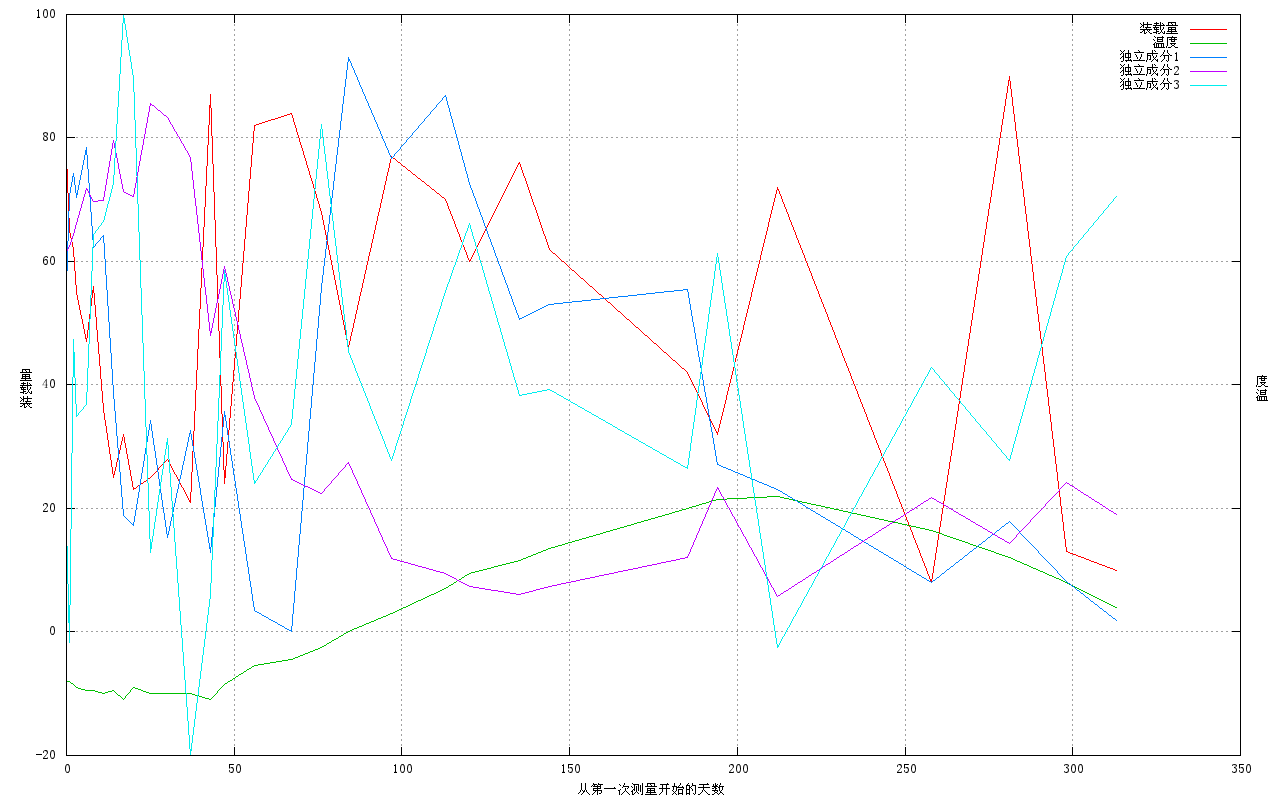
\includegraphics[scale=0.3]{42-pca-plot.png}
   \bicaption[figure:plot-42-pca]{二号末煤仓PCA降维后使用FastICA后得到的四个独立分量及装载量、气温的图像}
				    {二号末煤仓使用PCA降维FastICA后得到的四个独立分量及装载量、气温的图像}
			{Fig.}{Four IC(With PCA first), Loadage and Temperature for Powder Bulker No.2}
\end{figure}

\subsection{各影响因子与所得独立成分的关系}
在根据fastica或者PCA之后的FastICA得到独立成分之后,
为了评估各个独立成分与煤仓装载量、温度变化、经历时间的相互关系,
同时采用Pearson相关系数、互信息、灰关联度作为度量。

%直接FastICA后得到四个独立成分和煤仓装载量之间的相关度量 
\begin{table}[!htb]
\begin{center}
\bicaption{直接使用FastICA得到的独立成分与装载量之间的关系(一号末煤仓)}
			{直接使用FastICA得到的独立成分与装载量之间的关系(一号末煤仓)}
			{Table.}{Relationship between Loadage and ICs from FastICA directly, No.1 of Powder Bulker}
\begin{tabular}{lccclccc}
\toprule
                		& 相关系数     				& 互信息      					&灰关联度 \\
\midrule
  独立成分1     	&  0.31045550206419115       	& 0.94230515613664989   	&    \\
  独立成分2     	&  nan          					& 3.493152145488611e-15   	&    \\
  独立成分3     	&  0.63203026974852217      	& 0.94230515613664989		&    \\
  独立成分4     	&  -0.13494294423250519    	& 0.9423051561366498		&    \\
 \bottomrule
\end{tabular}
\end{center}
\end{table}

\begin{table}[!htb]
\begin{center}
\bicaption{直接使用FastICA得到的独立成分与装载量之间的关系(二号末煤仓)}
			{直接使用FastICA得到的独立成分与装载量之间的关系(二号末煤仓)}
			{Table.}{Relationship between Loadage and ICs from FastICA directly, No.2 of Powder Bulker}
\begin{tabular}{lccclccc}
\toprule
                		& 相关系数     				& 互信息      					&灰关联度 \\
\midrule
  独立成分1     	&  -0.0098565966362569018  	& 0.97325847231868035   	&    \\
  独立成分2     	&  0.64991952670167907		& 0.97325847231868035   	&    \\
  独立成分3     	&  0.27993093051194867      	& 0.9732584723186803		&    \\
  独立成分4     	&  -0.048345889699784657    	& 0.97325847231868035		&    \\
 \bottomrule
\end{tabular}
\end{center}
\end{table}

%直接FastICA后得到四个独立成分和气温之间的相关度量
\begin{table}[!htb]
\begin{center}
\bicaption{直接使用FastICA得到的独立成分与气温之间的关系(一号末煤仓)}
		{直接使用FastICA得到的独立成分与气温之间的关系(一号末煤仓)}
			{Table.}{Relationship between Temperature and ICs from FastICA directly, No.1 of Powder Bulker}
\begin{tabular}{lccclccc}
\toprule
                & 相关系数     						& 互信息      						&灰关联度 \\
\midrule
  独立成分1     &  -0.79715083668276143     	& 0.92753315430712713			&    \\
  独立成分2     &  nan							& 3.3089362752306921e-15		&    \\
  独立成分3     &  -0.0046455198649242432		& 0.92753315430712824 			&    \\
  独立成分4     &  -0.12419823845502126		& 0.92753315430712857 			&    \\
 \bottomrule
\end{tabular}
\end{center}
\end{table}

\begin{table}[!htb]
\begin{center}
\bicaption{直接使用FastICA得到的独立成分与气温之间的关系(二号末煤仓)}
		{直接使用FastICA得到的独立成分与气温之间的关系(二号末煤仓)}
			{Table.}{Relationship between Temperature and ICs from FastICA directly, No.2 of Powder Bulker}
\begin{tabular}{lccclccc}
\toprule
                & 相关系数     						& 互信息      						&灰关联度 \\
\midrule
  独立成分1     &  0.33269827762973381	     	& 0.92753315430712879			&    \\
  独立成分2     &  -0.11181095960366073		& 0.92753315430712746			&    \\
  独立成分3     &  0.84894488520244671		& 0.9275331543071224 			&    \\
  独立成分4     &  0.046542855465477796		& 0.92753315430712779			&    \\
 \bottomrule
\end{tabular}
\end{center}
\end{table}

%直接FastICA后得到四个独立成分和时间之间的相关度量
\begin{table}[!htb]
\begin{center}
\bicaption{直接使用FastICA得到的独立成分与时间之间的关系(一号末煤仓)}
		{直接使用FastICA得到的独立成分与时间之间的关系(一号末煤仓)}
			{Table.}{Relationship between Days and ICs from FastICA directly, No.1 of Powder Bulker}
\begin{tabular}{lccclccc}
\toprule
                		& 相关系数     					& 互信息      					&灰关联度 \\
\midrule
  独立成分1     	&  -0.67039265728626118     		& 0.99999999999824107   	&    \\
  独立成分2     	&  nan          						& 4.0089740251131844e-15   	&    \\
  独立成分3     	&  -0.26336501825181907      		& 0.99999999999824218   	&    \\
  独立成分4     	&  -0.23270816025544519      		& 0.99999999999824252  	&    \\
 \bottomrule
\end{tabular}
\end{center}
\end{table}

\begin{table}[!htb]
\begin{center}
\bicaption{直接使用FastICA得到的独立成分与时间之间的关系(二号末煤仓)}
		{直接使用FastICA得到的独立成分与时间之间的关系(二号末煤仓)}
			{Table.}{Relationship between Days and ICs from FastICA directly, No.2 of Powder Bulker}
\begin{tabular}{lccclccc}
\toprule
                		& 相关系数     					& 互信息      					&灰关联度 \\
\midrule
  独立成分1     	&  0.51625222015459338     		& 0.99999999999824285   	&    \\
  独立成分2     	&  -0.28080031928822285		& 0.99999999999824141   	&    \\
  独立成分3     	&  0.68571871171874499      		& 0.99999999999824307   	&    \\
  独立成分4     	&  -0.113386396661022      		& 0.99999999999824196  	&    \\
 \bottomrule
\end{tabular}
\end{center}
\end{table}

%首先使用PCA降维再使用FastICA后得到三个独立成分和煤仓装载量之间的相关度量
\begin{table}[!htb]
\begin{center}
\bicaption{PCA降维后使用FastICA得到的独立成分与装载量之间的关系(一号末煤仓)}
		{PCA降维后使用FastICA得到的独立成分与装载量之间的关系(一号末煤仓)}
			{Table.}{Relationship between Loadage and ICs from FastICA after PCA, No.1 of Powder Bulker}
\begin{tabular}{lccclccc}
\toprule
                		& 相关系数     					& 互信息      						&灰关联度 \\
\midrule
  独立成分1     	&  0.2635564858132709     		& 0.94230515613664989   		&    \\
  独立成分2     	&  0.3483940146795545			& 0.94230515613664989  		&    \\
  独立成分3     	&  0.62976934113327743			& 0.94230515613664989			&    \\
 \bottomrule
\end{tabular}
\end{center}
\end{table}

\begin{table}[!htb]
\begin{center}
\bicaption{PCA降维后使用FastICA得到的独立成分与装载量之间的关系(一号末煤仓)}
		{PCA降维后使用FastICA得到的独立成分与装载量之间的关系(一号末煤仓)}
			{Table.}{Relationship between Loadage and ICs from FastICA after PCA, No.1 of Powder Bulker}
\begin{tabular}{lccclccc}
\toprule
                		& 相关系数     					& 互信息      						&灰关联度 \\
\midrule
  独立成分1     	&  0.25118155055662922     		& 0.97325847231868035   		&    \\
  独立成分2     	&  -0.36213168393230483		& 0.97325847231868035  		&    \\
  独立成分3     	&  -0.35052673089969216		& 0.97325847231868035			&    \\
 \bottomrule
\end{tabular}
\end{center}
\end{table}

%首先使用PCA降维再使用FastICA后得到三个独立成分和气温之间的相关度量
\begin{table}[!htb]
\begin{center}
\bicaption{PCA降维后使用FastICA得到的独立成分与气温之间的关系(一号末煤仓)}
			{PCA降维后使用FastICA得到的独立成分与气温之间的关系(一号末煤仓)}
			{Table.}{Relationship between Days and ICs from FastICA after PCA, No.1 of Powder Bulker}
\begin{tabular}{lccclccc}
\toprule
                & 相关系数     				& 互信息      			&灰关联度 \\
\midrule
  独立成分1     &  -0.82599874780257931		& 0.92753315430712724   &     \\
  独立成分2     &  0.028941710801729584		& 0.92753315430712802   &     \\
  独立成分3     &  0.063245341965641827		& 0.92753315430712824   &      \\
 \bottomrule
\end{tabular}
\end{center}
\end{table}

\begin{table}[!htb]
\begin{center}
\bicaption{PCA降维后使用FastICA得到的独立成分与气温之间的关系(二号末煤仓)}
			{PCA降维后使用FastICA得到的独立成分与气温之间的关系(二号末煤仓)}
			{Table.}{Relationship between Days and ICs from FastICA after PCA, No.2 of Powder Bulker}
\begin{tabular}{lccclccc}
\toprule
                & 相关系数     				& 互信息      			&灰关联度 \\
\midrule
  独立成分1     &  -0.07804130719348294		& 0.92753315430712802	&    \\
  独立成分2     &  -0.85050833400604609		& 0.92753315430712802	&    \\
  独立成分3     &  -0.048183316293294788		& 0.92753315430712902	&    \\
 \bottomrule
\end{tabular}
\end{center}
\end{table}


%首先使用PCA降维再使用FastICA后得到三个独立成分和时间之间的相关度量
\begin{table}[!htb]
\begin{center}
\bicaption{PCA降维后使用FastICA得到的独立成分与时间之间的关系(一号末煤仓)}
		{PCA降维后使用FastICA得到的独立成分与时间之间的关系(一号末煤仓)}
			{Table.}{Relationship between Days and ICs from FastICA after PCA, No.1 of Powder Bulker}
\begin{tabular}{lccclccc}
\toprule
                & 相关系数     					& 互信息      					&灰关联度 \\
\midrule
  独立成分1     &  -0.68223727564185688  	& 0.9999999999982413   		&    \\
  独立成分2     &  -0.2629624823357441	      	& 0.99999999999824196   	&    \\
  独立成分3     &  -0.090631387884062373	& 0.99999999999824218   	&    \\
 \bottomrule
\end{tabular}
\end{center}
\end{table}

\begin{table}[!htb]
\begin{center}
\bicaption{PCA降维后使用FastICA得到的独立成分与时间之间的关系(二号末煤仓)}
		{PCA降维后使用FastICA得到的独立成分与时间之间的关系(二号末煤仓)}
			{Table.}{Relationship between Days and ICs from FastICA after PCA, No.1 of Powder Bulker}
\begin{tabular}{lccclccc}
\toprule
                & 相关系数     					& 互信息      					&灰关联度 \\
\midrule
  独立成分1     &  -0.38708135633534102  	& 0.99999999999824218 		&    \\
  独立成分2     &  -0.7471217157090686	      	& 0.99999999999824218   	&    \\
  独立成分3     &  0.042564507273735043	& 0.99999999999824329   	&    \\
 \bottomrule
\end{tabular}
\end{center}
\end{table}

\subsection{对以上结果的分析}
通过分析以上的图表,对比装煤量、当地平均气温、观测时间等信息,
比较图中的四个分量,可以得出结论:\\
    1) 煤仓刚投入使用的时候,各分量变化比较混乱。\\
    2) 后期各分量与装载量、温度、时间的关系开始变得比较明显,
	这可能是因为前期的操作不规范引起的。但是因为能获得的数据比较短,
	甚至没有达到一周年,结果显得比较混乱。\\
    3) 如果去掉前期数据,只使用后期的数据,结果或许会变得比较好一些。\\
    4) 虽然有以上的各个限制因素,但是还是可以很明显得看出装载量对沉降的影响最大,
	而温度和时间并不特别明显。这也可以说明,煤仓是安全的。\\
    5) 从上边可以看出,互信息并没有给出特别有用的信息,
	相对来说,还是相关系数可以更好地用来分析各种因素与各独立成分之间的关系。\\













